%%% EPS notes.

\documentclass{momento}

\usepackage{danielphysics}
%\usepackage{wasysym}
\title{Exploring Planetary Systems}
\author{Daniel Williams}

% \usepackage{zref-xr}
% \externaldocument{/home/astronomy/grg/project}

\providecommand{\Lag}{\mathcal{L}} %The Lagrangian

\begin{document}
\maketitle

\tableofcontents

These notes are based on the \textit{Exploring Planetary Systems}
course taught at the Unviersity of Glasgow during the 2014--2015
session.

\part{Spaceflight}
\label{part:spaceflight}

\chapter{The Rocket Equation}
\label{cha:rocket-equation}

\section{Derivation of the rocket equation}
\label{sec:deriv-rock-equat}

In order to change its momentum a rocket ejects mass; the Tsiolkovsky
rocket equation relates the complications of the changing mass and the
rocket's dynamics.  To analyse the motion of the rocket we start at
Newton's second law,
\begin{equation}
  \label{eq:10}
  \sum_i F_i = \dv{p(t)}{t}
\end{equation}
In the case of a rocket both the mass and the momentum have a time
dependence, and
\begin{equation}
  \label{eq:11}
  \dv{p}{t} = \lim_{\Delta t \to 0} \qty( \frac{p_2 - p_1}{\Delta t} )
\end{equation}
Consider $p_1 = (m + \Delta m) V$, and $p_2 = m(V + \Delta v) + \Delta
m V~e$, where $V~e$ is the velocity of the exhausted mass.

In the frame of an observer,
\[ V~e = V - v~e \]
thus 
\begin{align*}
  p_2 - p_1 &= m(V + \Delta v) + \Delta m (V-v~e) - (m+\Delta m) V \\
&= m \Delta v - \Delta m \ v~e
\end{align*}
let $\dd{m} = -\Delta m$, so
\begin{align*}
  \dv{p}{t} &= \frac{m \Delta v + v~e \dd{m}}{\Delta t} \\
&= m \dv{v}{t} + v~e \dv{m}{t} = m \dot{v} + v~e \dot{m}
\end{align*}
Since there are no external forces, and assuming that $v~e$ is
constant,
\begin{align*}
  F &= m \dot{v} + v~e \dot{m} = 0 \\
m \dot{v} &= - v~e \dot{m} \\
\Delta v &= \int v~e m \dd{m} 
\end{align*}
which gives
\begin{fequation}[Tsiolkovsky rocket equation]
  \label{eq:13}
\label{eq:rocket-equation}
  \Delta v= v~e \log( \frac{m_0}{m(t)} )
\end{fequation}
Now define the mass fraction as the proportion of the propellant which
has been expended,
\begin{definition}[Mass fraction]
  \label{def:mass-fraction}
  \[ M~f = 1 - \qty[ \frac{m(t)}{m_0}] \]
\end{definition}

\section{Thrust}
\label{sec:thrust}

If we make the assumption that $\dot{m}$ is constant, then
\[ m(t) = m_0 - \dot{m} t \]
and the total time for driven flight can then be found,
\begin{equation}
  \label{eq:14}
  t = \frac{m_0 - m(t)}{\dot{m}} = \frac{m_0}{\dot{m}} \qty( 1 - \frac{m}{m_0}) = \frac{m_0}{\dot{m}} M~f
\end{equation}
hence the range of the rocket is
\begin{align*}
  s(t) &= \int_0^t v(t') \dd{t'}\\ &= v~e \int_0^t \log( \frac{m_0}{m_0 - \dot{m} t'} ) \dd{t'} \\ &= v~e \frac{m_0}{\dot{m}}
\qty[\qty(1- \frac{\dot{m} t}{m_0}) \log( 1 - \frac{\dot{m} t}{m_0}) + \frac{\dot{m}}{m_0} t]\\
& \text{since } m(t) = m = m_0 - \dot{m} t, 1- \dot{m} t / m_0 = m(t)/m\\
&= v~e \frac{m_0}{\dot{m}} \qty[ \frac{m}{m_0} \log( \frac{m}{m_0}) +  1 - \frac{m}{m_0}] \\ 
&= v~e \frac{m_0}{\dot{m}} \qty[ 1 - \frac{m}{m_0} \qty( \log(\frac{m}{m_0}) + 1 )]
\end{align*}

\section{Equations of motion}
\label{sec:equations-motion}

We now have a set of equations to describe the rocket's motion,
\begin{align}
  \label{eq:15}
  v(t) &= v~e \log( \frac{m_0}{m} ) \\
  \label{eq:16}
  t &= \frac{m_0}{\dot{m}} M~f \\
  \label{eq:17}
  s(t) &= v~e \frac{m_0}{\dot{m}} \qty[1 - \frac{m}{m_0} \qty(\log( \frac{m}{m_0} )+1)] + v_i \frac{m_0}{\dot{m}} M~f
\end{align}

It is useful to define a new quantity here also:
\begin{definition}[Specific Impulse]
\label{def:specific-impulse}
  \[ I~{sp} = \frac{v~e}{g} \]
\end{definition}
which is just the exhaust velocity normalised by the gravitational
acceleration.

\begin{example}[A simple rocket]
  Consider the third stage burn of a rocket, which has an initial
  velocity $v~i = 2 \e{3}\, \meter\, \second^{-1}$, and contains $4
  \e{3}\, \kilogram$ of fuel, and has an empty mass of $700\,
  \kilogram$. The vacuum exhaust speed is $v~e =
  2930\,\meter\,\second^{-1}$, with
  $\dot{m}=100\,\kilogram\,\second^{-1}$. \\ How far does the rocket
  travel during the burn?  The mass ratio is $\frac{4.7}{0.7} =
  6.71$, so \[ \Delta v = v~e \log(6.71) =
  55.79\,\meter\,\second^{-1} \] and the burn time is
\[ \Delta t = \frac{4.7}{0.1 (1 - \frac{0.7}{4.7} )} \approx 40\,\second \]
Thus \begin{align*} s &= 2930\,\meter\second^{-1} &&\times \frac{4700\,\kilogram}{100\,\kilogram\,\second^{-1}}\\ &&& \times \qty[1 - \frac{1}{6.71} \qty( \log(6.71) + 1 )] \\&= 158.51 \kilo\meter 
\end{align*}
\end{example}

\section{Multistaging}
\label{sec:multistaging}

The structural mass of the rocket is a major source of inefficiency
during the burn, and one way to reduce its impact is to jettison
stages of the rocket as the fuel they are carrying is expended. This
allows a greater speed to be achieved with the same quantity of
fuel. Modern rockets seldom use more than three stages due to the
engineering compexity, however.

From the rocket equation (\ref{eq:rocket-equation}), we have
\[ v(t) = v~E \log( \frac{M_0}{M} ) + v~i \] for $M_0$ the initial
mass of the rocket, and $M$ its final mass, while $v~i$ is its
velocity at the start of the burn. For a single stage rocket the
velocity boost will be
\[ v(t) = v~E \log(R_0) \]
where 
\[ R_0 = \frac{M~S + M~f + M~p}{M~s + M~p} \] for $M~S$, $M~f$, and
$M~p$ respectively the masses of the structure, fuel, and payload.

If the rocket is composed of two stages with equal mass,
\[ v(t) = v~E \log(R_1) + v~E \log(R_2) \] which is larger than the
total speed achievable using a single-stage rocket.

%%% Local Variables: 
%%% mode: latex
%%% TeX-master: "../project"
%%% End: 


\chapter{Rocket Launches}
\label{cha:rocket-launches}

\section{Vertical motion against gravity}
\label{sec:vert-moti-against}

Consider a rocket with thrust velocity perpendicular to the
gravitational field. The force equation  is
\begin{equation}
  \label{eq:1}
  \dv{v}{t}= \frac{F-Mg}{M}
\end{equation}
For $Mg$ the instantaneous weight of the rocket. Hence
\begin{equation*}
  \label{eq:2}
  \dv{v}{t} = -v~E \frac{\dot{M}}{M}-g
\end{equation*}
then
\begin{equation*}
  \dd{v} = - v~E \frac{\dd{M}}{M} - g \dd{t}
\end{equation*}
and integrating both parts from $t=0$ to $t$,
\begin{equation*}
  v(t) = - v~E \int_{M_0}^M \frac{\dd{M'}}{M'} - \int_0^t g \dd{t'}
\end{equation*}
Assuming that $g$ is constant over the flight,
\begin{align*}
  v(t) &= v~E \log( \frac{M_0}{M(t)} )-gt \\
&= v~E \log(\frac{M_0}{M(t)}) - g \frac{M_0}{\dot{M}} \qty( 1 - \frac{M}{M_0})
\end{align*}
with the second part of the equation the gravity loss term.

\section{Thrust-to-weight ratio}
\label{sec:ttw-ratio}

In order to optimise the amount of energy lost due to gravity we can
consider the \emph{thrust-to-weight ratio}, 
\begin{equation}
  \label{eq:3}
  \psi = \frac{F}{g M_0} = \frac{v~E \dot{M}}{g M_0}
\end{equation}
which allows us to write
\begin{equation}
  \label{eq:4}
  \frac{v(t)}{v~E} = \log( \frac{M_0}{M(t)} ) - \frac{1}{\psi} \qty( 1 - \frac{M}{M_0} )
\end{equation}

\section{Vertical range}
\label{sec:vertical-range}

To calculate the vertical range of a rocket we proceed as before by
integrating the velocity over $t$
\begin{align*} 
s &= \int v(t) \dd{t} = v~E \int_0^t \log( \frac{M_0}{M(t)} ) \dd{t} - \int_0^t g t \dd{t'} \\
&=v~E \frac{M_0}{\dot{M}} \qty[ 1 - \frac{M}{M_0} \qty( \log( \frac{M_0}{M(t)}) + 1 ) ] - \half g t^2 \\
&=v~E \frac{M_0}{\dot{M}} \qty[ 1 - \frac{M}{M_0} \qty( \log( \frac{M_0}{M(t)}) + 1 ) ] \\ & \quad- \frac{g}{2} \frac{M_0^2}{\dot{M}^2} \qty( 1 - \frac{M}{M_0})^2
\end{align*} assuming $g$ is constant.

\section{Launch aspects}
\label{sec:launch-aspects}

Consider the kinetic energy of the payload,
\begin{align*}
  \half M \Delta v^2 &= \half M v~E^2 \log^2\qty(\frac{M_0}{M}) \\ &= \half M v~E^2 \log^2\qty(R)
\end{align*}
For $R$ the rocket parameter. Normalising this by the rest-frame
energy of the propellant in the rocket,
\[ \half (M_0-M) v~E^2 \]
we find the ratio
\begin{equation}
\label{eq:5} \phi(R) = \frac{M}{M_0-M} \log^2(R) = \frac{\log^2(R)}{R-1} 
\end{equation}

\begin{figure}[b]
  \centering
  \begin{tikzpicture}
    \begin{axis}[xmin=0, ymin=0, height = 5cm, width=\columnwidth, xlabel=$R$, ylabel=$\phi(R)$]
      \addplot[mark=none, draw=muted-green, ultra thick, domain=1:10] {(ln(x)*ln(x))/(x-1)};
    \end{axis}
  \end{tikzpicture}
  \caption{$\phi(R)$ as a function of the rocket parameter, $R$.}
  \label{fig:rocket-ratio}
\end{figure}

By differentiating we find the optimal $R$ to be
\begin{equation}
  \label{eq:6}
  \dv{\phi}{R} = 0 = - \frac{\log^2(R)}{(R-1)^2} + \frac{2 \log(R)}{R(R-1)}
\end{equation}
So the optimal $R = R~C$ satisfies
\begin{equation}
  \label{eq:7}
  \log{R~C} = 2 - \frac{2}{R~C}
\end{equation}
so $R~C \approx 4.9$.

It is also important that the payload obtains a horizontal speed in
order to remain in orbit. This requires an inclined launch, with two
components of motion,
\[
\dv{v_z}{t} = \frac{F \sin(\theta)-Mg}{M}, \qquad \dv{v_x}{t} = \frac{F \cos(\theta)}{M} 
\]
for $\theta$ the pitch angle from $\theta=0$ horizontal. Thus
\begin{align*}
v_z(t) &= v~E \sin(\theta) \log( \frac{M~0}{M~E} ) - gt \\ v_x(t) &= v~E \cos(\theta) \log(\frac{M_0}{M})
\end{align*}
assuming $v(0)=0$. The total speed of the rocket is then
\begin{align*}
 v(t) &= \sqrt{v^2_x + v^2_z} \\ &= \qty( v~E^2 \qty( \log(\frac{M_0}{M}))^2 - 2 v~E g t \sin(\theta) \log( \frac{M_0}{M}) + g^2 t^2 )^{\half} 
\end{align*}

The path angle of the flight is related to the ratio of the vertical
to the horizontal velocity, so
\begin{align*} \tan(\gamma) &= \frac{v~E \sin(\theta) \log(\frac{M_0}{M})-gt}{v~E \cos(\theta) \log(\frac{M_0}{M})} \\
&= \tan(\theta) - \frac{gt}{v~E \cos(\theta) \log( \frac{M_0}{M})} \\
& \approx \tan(\theta) - \frac{g M_0}{v~E \dot{M} \cos(\theta)} \quad \text{early in flight}
\end{align*}

We can define the angle of attack as the angle between the thrust and
the flight path, which tends to zero as the burn progresses.

The drag, $F~D$, and lift, $F~L$, are
\[ F~D = C~D A \frac{\rho v^2}{2}, \qquad F~L = C~L A \frac{\rho v^2}{2} \]
where 
\[ \frac{\rho v^2}{2} \] is the dynamic pressure, $C~D$ the drag
coefficient, $C~L$ the lift coefficient, and $A$ the cross-sectional
area.


\section{The gravity turn}
\label{sec:gravity-turn}

A gravity turn is used to rotate the angle of a trajectory using the
gravitational effect of the Earth. Consider the equations from earlier for a constant pitch angle, but substitute the flight path angle, $\gamma$ for the pitch angle, $\theta$, so
\begin{align*}
  \dv{v_z}{t} &= \frac{F}{M} \sin(\gamma) - g = \frac{F}{M} \frac{v_z}{v} -g \\
\dv{v_x}{t} &= \frac{F}{M} \cos(\gamma) =\frac{F}{M} \frac{v_x}{v}
\end{align*}
then multiplying each by their respective velocities, and summing them,
\[ v_z \dv{v_z}{t} + v_x \dv{v_x}{t} = v \dv{v}{t} = \frac{F v}{M} - gv_z \]
Then, the expression for $v$ becomes
\[ \dv{v}{t} = \frac{F}{M} - g \frac{v_z}{v} = \frac{F}{M} - g \sin(\gamma) \]
Multiplying $\dv{v_x}{t}$ by $v_z$ and vice versa, then subtracting one from the other,
\[ v_x \dv{v_z}{t} - v_z \dv{v_x}{t} = - g v_x \]
Since $\tan(\gamma) = v_z / v_x$,
\[ \dv{t} \tan(\gamma) = \frac{\dot{v}_z}{v_x} - \frac{v_z \dot{v}_x}{v_x^2} = \frac{v_x \dot{v}_z - v_z \dot{v}_x}{v_x^2} \]
and the left hand side can be rewritten
\[ \dot{\gamma} (1-\tan[2](\gamma) ) = \dot{\gamma} \qty( 1+ \frac{v_z^2}{v_x^2} ) = \dot{\gamma} \frac{v^2}{v^2_x} \]
Thus, combined,
\[ \dv{\gamma}{t} = - \frac{g v_x}{v^2} = - \frac{g}{v} \cos(\gamma) \]

The equations governing the flight path are non-linear, so some
simplifications are required to solve them.

\section{A uniformly changing path angle}
\label{sec:unif-chang-path}

Suppose $\dot{\gamma} = -C$ is constant, so $\gamma$ changes uniformly
with time. Then
\[ C = \frac{g}{v} \cos(\gamma) \]
so
\[ \dot{v} = - \frac{g}{C} \sin(\gamma) \dot{\gamma} = g \sin(\gamma) \]
Thus
\[ \dot{v} = \frac{F}{M} - \dot{v} \implies 2 \dot{v} = \frac{F}{M} \]
So
\[ \dot{v} = \frac{F}{2M} = \half v~E \frac{\dot{M}}{M} \]
which has a solution
\[ v(t) = v_0 + \half v~E \log(\frac{M_0}{M}) \]
Which, given $\cos(\gamma) = Cv/g$,
\begin{equation}
  \label{eq:58}
  \cos(\gamma(t)) = \cos(\gamma_0) + C \frac{v~E}{2 g} \log(\frac{M_0}{M})
\end{equation}

\section{Orbital injection}
\label{sec:orbital-injection}

Once the atmosphere is sufficiently tenuous orbital injection can
occur, with the perigee of the orbit an important deciding parameter.
For a circular orbit,
\[ v = \sqrt{\frac{GM}{R}+h} \]
and for a parabolic orbit
\[ v = \sqrt{\frac{2GM}{R} + h} \] with everything in between being an
elliptical orbit.

%%% Local Variables: 
%%% mode: latex
%%% TeX-master: "../project"
%%% End: 


\chapter{Orbits \& Manoeuvres }
\label{cha:orbits}

\chapter{Rocket Engines}
\label{cha:rocket-engines}

\chapter{New Propulsion Methods}
\label{cha:new-prop-meth}



\part{Space Exploration}
\label{part:space-exploration}

\chapter{Detecting Exoplanets}
\label{cha:detecting-exoplanets}

A planet is an object which orbits a star or a stellar remnant,
defined in 2006 by the IAU as celestial body which
\begin{itemize}
\item is in orbit around the Sun,
\item has sufficient mass for its self-gravity to overcome rigid body
  forces so that it assumes a hydrostatic equilibrium (nearly round)
  shape, and
\item has cleared the neighbourhood around its orbit.
\end{itemize}
an exoplanet is a planet in orbit about a star other than our own.

The earliest attempts to detect exoplanets came from Huygens in 1698,
while the first successful detection was made in 1992, with the
discovery of a planet orbiting a pulsar. The first main sequence star
found to have planets was 50 Persei in 1995.

There are a number of methods used to detect exoplanets:

\begin{description}
\item[Direct observation] Planets are identified by the reflected
  radiation, either through optical, infra-red, or radio emission, and
  its polarisation.
\item[Doppler Method] Radial velocity changes of the star with respect
  to the Earth can be deduced from the star's spectral lines.
\item[Astrometry] By measuring the position of a star in the sky the
  'wobble' in the star's relative motion caused by the planet can
  reveal the presence of planets.
\item[Transit Method] The effect of the planet on the observed
  luminosity of a star as it passes in front of the disk can be
  measured.
\item[Gravitational Microlensing] The gravitational field of a star
  acts like a lens, brightening the background stars.
\item[Pulsar Timing] The presence of a planet introduces a delay in
  the arrival of pulses.
\end{description}

\section{Direct Observation}
\label{sec:direct-observation}

\subsection{Albedo}
\label{sec:albedo}

The albedo is the ability of an object to reflect light. \\
Let the radiation flux density on the surface of the Sun be $F~\sun$,
and so the flux density, $F~p(r)$ at a distance $r$ from the star is
\begin{equation}
  \label{eq:1}
  F~p(r) = F~\sun \frac{R^2_{\sun}}{r^2}
\end{equation}
with $R_{\sun} /\ r$ being the angular diameter of the Sun at a
distance $r$. Then the total flux on the surface of the planet then becomes 
\[ L = \pi R^2~p F~p = \pi R^2~p F_{\sun} \frac{R^2_{\sun}}{r^2} \]

\subsection{Bond Albedo}
\label{sec:bond-albedo}

The Bond Albedo, $A$, is defined as the ratio of the emergent flux to
the incident flux. The flux reflected by the planet is

\begin{equation}
  \label{eq:2}
  L = L^{\prime} \cdot A =  \pi R^2~p A F_{\sun} \frac{R^2_{\sun}}{r^2}
\end{equation}

If a planet is a distance $\Delta$ from the observer its observed
flux, $F$, will be
\begin{equation}
  \label{eq:3}
  F = \frac{L^{\prime}}{4 \pi \Delta^2}
\end{equation}

However, reflection is anisotropic, so the flux must be corrected by a
factor $C \Phi(\alpha)$ which depends on the phase angle of the
planet. The function $\Phi$ is the phase function, and is normalised
such that $\Phi(\alpha = 0) = 1$. We also require the normalising
constant $C$ such that
\begin{equation}
  \label{eq:4}
  \frac{ C \int_S \Phi(\alpha) \dd{S}}{4 \pi \Delta^2} = 1
\end{equation}

With this, the true observed flux at a distance $\Delta$ will be
\begin{equation}
  \label{eq:5}
  F = \frac{C \Phi(\alpha) L^{\prime}}{4 \pi \Delta^2} 
    = \frac{C \Phi(\alpha)}{4 \pi \Delta^2} A \pi R^2~p F_{\sun} \frac{R_{\sun}^2}{r^2}
\end{equation}

Now, since
\begin{align*}
  \int_S \Phi(\alpha) \dd{S} & = \Delta^2 \int_{\alpha=0}^{\pi} \int_{\phi=0}^{2\pi} \Phi(\alpha) \sin(\alpha) \dd{\alpha} \dd{\phi} \\
                             & = 2 \Delta^2 \pi \int_0^{\pi} \Phi(\alpha) \sin(\alpha) \dd{\alpha}                                   \\
  \therefore C               & = \frac{2}{\int_0^{\pi} \Phi(\alpha) \sin(\alpha) \dd{\alpha}}
\end{align*}

Let $q = \frac{CA}{4}$. The Bond Albedo, $A$, can be expressed
\begin{equation}
  \label{eq:6}
  A = 2 p \int_{\alpha=0}^{\pi} \Phi(\alpha) \sin(\alpha) \dd{\alpha}
\end{equation}
with $p$ the geometric albedo, and $q$ is the phase integral:
\begin{equation}
  \label{eq:7}
  q = 2 \int_{\alpha=0}^{\pi} \Phi(\alpha) \sin(\alpha) \dd{\alpha}
\end{equation}

\subsection{Geometric Albedo}
\label{sec:geometric-albedo-1}

A Lambertian surface is a perfectly white diffuse surface which
reflects all incident radiation, with a phase function $\Phi(\alpha) =
\cos(\alpha)$. Thus
\begin{equation}
  \label{eq:8}
  C = \frac{2}{\int_0^{\pi} \Phi(\alpha) \sin(\alpha) \dd{\alpha}} 
    = \frac{2}{\int_0^{\pi/2} \cos(\alpha) \sin(\alpha)  \dd{\alpha} } = 4
\end{equation}
which implies that $A = p = 1$ for a Lambertian surface.

We can then use a Lambertian surface to measure the amount of light
reflected from another surface.  Take the observed flux density,
equation (\ref{eq:5}), and let $\alpha=0$. Now take the flux density
of the Lambertian surface,
\begin{equation}
  \label{eq:9}
  F~L(\alpha=0) = \frac{4}{4 \pi \Delta^2} \pi R~p^2 F_{\sun} \frac{R_{\sun}^2}{r^2} 
\end{equation}
since $A=1$. The ratio of these two gives $\frac{F}{F~L} = p$.

\section{Astrometric detection}
\label{sec:astr-detect}

As a planet orbits a star the mutual gravitational force causes the
two to orbit a mutual barycentre, and as such, the star appears to
wobble from side to side. The motion of a single planet about a star
causes the star to undergo a reflex circular orbit about the
barycentre with a radius
\[ a~s = a \frac{M~p}{M~s} \] This results in periodic perturbation of
the radial velocity, astrometric position, and time of arrival of
periodic signals.

The Keck telescopes are capable of detecting the position of a star to
within $20\,\micro\text{as}$, which allows the barycentric motion to
be detected. The radius of the orbit about the barycentre for the star is
\begin{equation}
  \label{eq:26}
  r~s = r \qty( \frac{m~p}{m~s + m~p} ) \approx r \qty( \frac{m~p}{m~s})
\end{equation}
Thus, at a distance $d$ this will produce an angular movement of 
\begin{equation}
  \label{eq:27}
  \Delta \theta = \frac{r~s}{d} = \frac{r}{d} \frac{m~p}{m~s}
\end{equation}
Defining the mass ratio, $q = m~p/m~s$, then
\begin{equation}
  \label{eq:28}
  \Delta \theta = 0.5 \qty( \frac{q}{10^{-3}}) \qty( \frac{r}{5\,\text{AU}} ) \qty( \frac{d}{10\,\text{pc}})^{-1} \,\milli\text{as}
\end{equation}
This method has the advantage of being able to estimate the mass of a
planet, and is complementary to the spectroscopic method, as it works
best for face-on systems. It is also ideal for detecting planets with
long orbital periods. On the other hand, achieving the required
precision is difficult, and the method is highly sensitive to the
distance to the parent star. There are also periodic shifts in a
star's apparent centroid position due to dark regions on its surface,
so long observation times are needed to confirm a detection.

\subsection{Surveys}
\label{sec:surveys-2}

\begin{description}
\item[Carnegie] The CAPSCam instrument at La Campanas, Chile has a
  $0.25\,\milli\text{as}/\text{hour}$ sensitivity, allowing a search
  for Jupiter-sized planets around the nearest 100 low-mass stars.
\item[GAIA] GAIA has a sensitivity of $25\,\micro\text{as}$ on average
  over its bandpass, and will monitor $1\e{9}$ stars, and can identify
  Jupiter-like planets at semi-major axes of $3\,\text{AU}$ and
  greater.
\end{description}

\section{Radial velocity}
\label{sec:radial-velocity}

In a system where the planet and star are, respectively at a distance
$r~p$ and $r~s$ from the barycentre the period will be
\[ P = \frac{2 \pi r~p}{v~p} = \frac{2 \pi r~s}{v~s} \] where $v~p$
and $v~s$ are the respective velocities. From conservation of momentum 
\[ M~p v~p = M~s v~s \] and so
\[ v~s = \frac{M~p}{M~s} \frac{2 \pi r~p}{P} \]
and since the line of sight may be inclined,
\[ v~r = v~s \sin(i) = \frac{M~p}{M~s} \frac{2 \pi r~p}{P} \sin(i) \]
is the radial velocity.

Recalling Kepler's third law,
\[ P^2 = \frac{4 \pi^2}{G(M~p + M~s)} r~p^3 \]
and so long as $M~p \ll M~s$,
\[ r~p \approx \qty( \frac{G M~s}{4 \pi^2} P^2 )^{\frac{1}{3}} \]
and therefore
\begin{equation}
  \label{eq:12}
  v~r = \qty( \frac{2 \pi G}{P})^{\frac{1}{3}} \frac{M~p}{M~s^{\frac{2}{3}}} \sin(i)
\end{equation}

The radial velocity can be measured from the Doppler shift of the
radiation from the star, and it is then possible to measure the
quantity $M~p \sin(i)$ for $i$ the inclination of the planet's
orbit. In the most general case the velocity amplitude, $K$, is
\begin{equation}
  \label{eq:18}
  K = \qty( \frac{2 \pi G}{P})^{\frac{1}{3}} \frac{M~p \sin(i)}{(M~p + M~s)^{\frac{2}{3}}} \frac{1}{(1-e^2)^{\half}}
\end{equation}
The star's mass can be estimated from the mass-luminosity
relationship, and once the distance to the star has been determined
(by parallax) the luminosity can be determined.

In absence of other constraints on the orbital inclination, radial
velocity searches can provide lower limits on the planetary masses of
a system. The magnitude of the radial velocity of the sun due to
Jupiter is around $12.5\,\meter/\second$, but due to the Earth is
$0.1\,\meter/\second$. The limit measurable by current instrumentation
is around $1\,\meter/\second$.

This method has the advantages of being independent of the distance to
the star, and the mass, period, and orbital elements of the planet can
be determined. It has the disadvantage of the inability to measure
$\sin(i)$ causing only the lower mass limit to be observable, thanks
to the SNR considerations around bright stars. Elliptical orbits
complicate the mathematics, as do multiple planet systems, and stellar
pulsations.

\subsection{Surveys}
\label{sec:surveys-1}

Three major radial velocity searches have been carried out.
\begin{description}
\item[HARPS] The High Accuracy Radial velocity Planetary Search is
  carried out by a spectrograph at Paranal, Chile, and is capable of
  detecting radial velocities as small as $\approx
  0.9\,\meter/\second$, which is sensitive to Earth-like
  planets. Gliese 581e was discovered by this survey, and is in a
  system orbiting a red dwarf 20\,ly away, with at least 6
  planets. The e planet is estimated to have a mass of around
  $1.7\,M~E$, while the g planet is in the habitable zone with a mass
  of $3.1\,M~E$.
\item[SOPHIE] This is a high resolution spectrograph at
  Haute-Provence, France, capable of observing radial velocities as
  small as $2\,\meter/\second$, and is used to follow-up Kepler
  objects of interest.
\item[Keck] The HIRES instrument on the Keck telescopes is attributed
  with having discovered more exoplanets than any other instrument
  prior to Kepler. It measures radial velocities around
  $1\,\meter/\second$.
\end{description}

\section{Planetary transits}
\label{sec:planetary-transits}

A growing number of extra-solar planets are detected by the transit
method, whereby the photometric effect of the planet passing over the
star's disk is recorded. The dip in intensity is related to the area
of the two disks,
\begin{equation}
  \label{eq:19}
  \Delta I \propto \qty( \frac{R~p}{R~s} )^2
\end{equation}
for $R~p$ the radius of the planet and $R~s$ the radius of the star,
so a planet the size of Jupiter is likely to cause a 1\% drop in
intensity, whereas the Earth would only produce a 0.01\% drop.

The reduction in brightness can be found as the ratio of the
brightness during the transit to that outside the transit.
\begin{equation}
  \label{eq:20}
  \frac{B~s \pi (R~s^2 - R~p^2)}{B~s \pi R~s^2} = 1 - \qty( \frac{R~p}{R~s} )^2
\end{equation}
for $B~s$ the brightness of the star, and the fractional change,
$\Delta$ is then
\begin{equation}
  \label{eq:21}
  \Delta = \qty( \frac{R~p}{R~s} )^2
\end{equation}

The first transit observed was of a planet around HD\,209458, which
had a 2.5\,hour transit time. This method allows the radius of the
planet to be measured easily, and allows a simultaneous scan of a
large fraction of the sky, and allows the atmospheres of planets, and
satellites, to be studied. It does however, require a good alignment
between the planets' orbital plane and the observer, and produces a
high rate of false detections.

In order to determine the orbital period we can turn to Kepler's third
law. The radius of the star can be estimated from the star's spectral
classification, allowing the planet's radius to be estimated. Along
with the mass of the star and the period it is possible to find the
planet's orbital radius.

\begin{figure}[b]
  \centering
  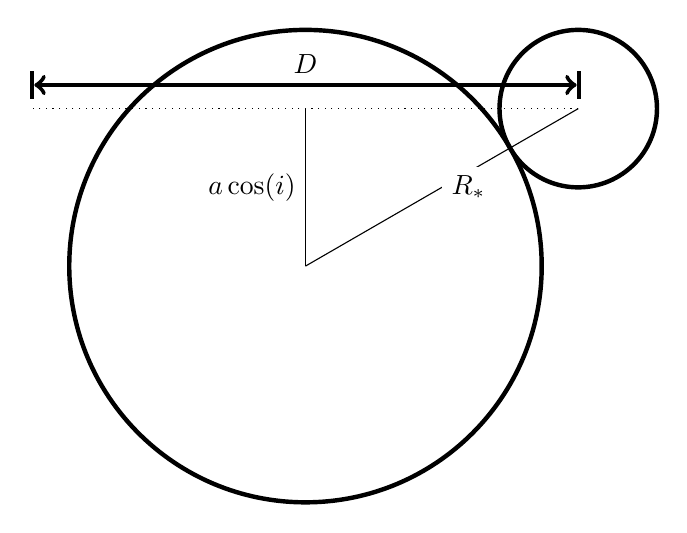
\begin{tikzpicture}[]
	\draw [ultra thick] ( 0,0) circle (3);
	\draw [ultra thick] (30:4) circle (1);
	\draw [dotted]   (30:4) -- (150:4);
	\draw [|<->|, ultra thick]     (-3.5, 2.3) -- (3.5,2.3) node [midway, above] {$D$};
	\draw (0, 0) -- (0,2) node [midway, left] {$a \cos(i)$};
	\draw (0,0) -- (30:4) node [midway, right, fill=white] {$R_*$};
\end{tikzpicture}
  \caption{The geometrical configuration of the transit.}
  \label{fig:transit-geometry}
\end{figure}

A transit will begin when the projected radius of the planet touches
the edge of the parent star, and lasts for a duration $\tau$ which is
a fraction of the total orbital period, and so the distance is a chord
of length
\begin{equation}
  \label{eq:22}
  D = 2 a \sin( \half \frac{2 \pi}{P} \tau) = 2 \sqrt{( R_{*} + R~p)^2 - a^2 \cos[2](i)}
\end{equation}
and so
\begin{equation}
  \label{eq:23}
  \tau = \frac{P}{\pi} \asin( \frac{\sqrt{(R_{*}+R~p)^2 - a^2 \cos[2](i)}}{a} )
\end{equation}
\begin{figure}[b]
  \centering
  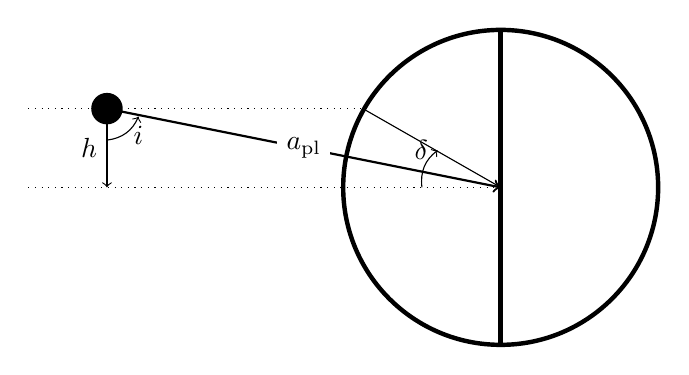
\begin{tikzpicture}[]
	\draw [ultra thick] (6,0) circle (2);
	\draw [ultra thick] (6,2) -- (6,-2);
	\draw [dotted]   (0,1) -- (4.25,1);
	\draw [dotted]   (0,0) -- (6,0);
	\draw [<->]      (1,0) -- (1,1) node [midway, left] {$h$};
	\fill (1,1) circle (0.2);
	\draw [thick, <->] (1,1) -- (6,0) node [midway,fill=white] {$a_{\rm pl}$};
	\draw [->] (1,0.6) to [bend right] (1.4,0.9) node [below] {$i$};
\draw (6,0) -- (4.25,1);
\draw [->] (5, 0) to [bend left] (5.2, 0.47) node [left] {$\delta$};
\end{tikzpicture}
  \caption{The transit geometry, side-on.}
  \label{fig:transit-geometry-2}
\end{figure}
This can also be described, using the geometry of figure
\ref{fig:transit-geometry-2} as
\begin{align*}
  \label{eq:24}
  \tau &= \frac{P}{\pi} \qty( \frac{R_{*} \cos(\delta) + R~p}{a} ) \\ &\approx 13 \qty( \frac{M_{*}}{M_{\odot}})^{-\half} \qty( \frac{1}{1\,\text{AU}} )^{\half} \qty( \frac{R_{*}}{R_{\odot}} )
\end{align*}
We find that the appropriate transit period is around 13 hours and 25
hours for Jupiter.

In order to view a transit the inclination of the system must
satisfy \[ \cos(i) \le \frac{(R~p + R~s)}{a} \] and the probability of
viewing a transit for the system is
\begin{equation}
  \label{eq:25}
  P(\text{transit}) = \frac{\int_0^{(R~p+R~s)/a} \dd{\cos(i)}}{\int_0^1 \dd{\cos(i)}} = \frac{R~p + R~s}{a} \approx \frac{R~s}{a}
\end{equation}

\subsection{Surveys}
\label{sec:surveys-3}

\begin{description}
\item[SuperWASP] This is the UK's leading wide-field exoplanet
  detection programme, which has been operating since 2004, and has
  discovered around 100 planets, using off-the-shelf Canon 200mm
  lenses, and science-grade CCDs.
\item[CoRoT] The Convection, Rotation, and Transits mission was
  dedicated to asteroseismology, and the discovery of exoplanets. It
  ran from 2006 to 2013, and detected 29 exoplanets.
\item[Kepler] Kepler has a specially-designed 0.95 meter mirror
  equipped for precise photometry, and by the end of 2014 had
  identified 989 planets, and an additional 4234 candidates.
\end{description}

\section{Gravitational microlensing}
\label{sec:grav-micr}

If a planet aligns precisely with the line-of-sight then the image of
the star will be deformed into a circle with a radius
\begin{equation}
  \label{eq:30}
  \theta~E = \sqrt{ \frac{4 G M~L}{c^2 D~L} \frac{(D~S - D~L}{D~S}} }
\end{equation}
This comes from the angle of deviation caused by the lens,
\begin{equation}
  \label{eq:29}
  \alpha = \frac{4 G M~L}{c^2 r} = \frac{2 R~s}{r}
\end{equation}
for $R~s$ the Shcwarzschild radius, and $r$ the distance of closest
approach, and $M~L$ is the mass of the lens. For a full derivation see
notes on \textsc{General Relativity} for more information.

The total magnification, $A$, which is produced is
\begin{equation}
  \label{eq:31}
  A = \frac{u^2 + 2}{u \sqrt{u^2 + 4}}
\end{equation}
where $u = \theta~s / \theta~E$ is a dimensionless unit representing
the source-lens separation in units of the Einstein radius. The
characteristic time of a lensing event is
\begin{equation}
  \label{eq:32}
  t~E = 69.9 \qty( \frac{M~L}{M_{\odot}} )^{\half} \qty( \frac{D~S}{8\,\kilo\text{pc}})^{\half} \qty[ (1-d)d]^{\half} v^{-1}_{200}\,\text{days}
\end{equation}

\textbf{A better description is contained in Dominik and Sahu, worth
  writing up from there.}

This method has the advantage of allowing the detection of Earth-like
planets, and allows a distribution of planetary systems to be
measured. Unfortunately lensing is a one-off process, and planets are
distant, so follow-up observations are implausible.

% \subsection{Surveys}
% \label{sec:surveys-4}

% A number of microlensing surveys have exoplanet detection as a main or secondary aim, including $\mu$FUN-PLANET, RoboNETII, MOA, and OGLE.

\section{Pulsar timing}
\label{sec:pulsar-timing}

By observing the timing residuals from pulsars it is possible to
distinguish periodic signals which correspond to orbiting bodies. The
first exoplanet discovered in this manner was in 1992 about the
millisecond pulsar PSR\,1257+12. Timing irregularities can be caused
by a number of effects other than just planets, however, including
seismic effects on the star, propagation effects, and other
relativistic effects.

A planet in a circular orbit will produce a timing residual of
\begin{equation}
  \label{eq:33}
  \tau~p = 1.2 \qty( \frac{M~p}{M~E} ) \qty( \frac{P}{1\,\text{year}})^{2/3}\,\milli\second
\end{equation}
which, combined with the inclination of the orbit allows a limit to be
placed on the mass,
\begin{equation}
  \label{eq:34}
  M~p \sin(i) \le 0.815 M~E \tau~p P^{-2/3}
\end{equation}

\subsection{The PSR\,1257+12 system}
\label{sec:psr-1257+12-system}

The first planetary system discovered around a pulsar was annnounced
in 1992 \cite{1992Natur.355..145W}, using a modified version of
\texttt{TEMPO} to fit out Keplerian orbital parameters in the TOAs
from the pulsar.
\begin{table}[b]
  \centering
  \begin{tabular}{l ccc}
\toprule
    Parameter        & Planet A  & B          & C          \\
\midrule
Semi-m axis (AU) & 0.19      & 0.36       & 0.46       \\
Mass ($M_{\oplus}$)  & 0.020     & 4.3        & 3.9        \\
Period (days)        & 25.262(3) & 66.5419(1) & 98.2114(2) \\
Eccentricity         & 0.0       & 0.0186(2)  & 0.0252(2)\\
\bottomrule
  \end{tabular}
  \caption{The orbital and physical parameters of the planets of the PSR\,1257+12 system. \cite{2003ApJ...591L.147K}}
  \label{tab:pulsar-planets}
\end{table}
The planets in the system are believed to have formed in a secondary
period of planet formation. The simplest model would be to assume that
the planets had survived not only the initial supernova which created
the pulsar, and its preceding red giant phase, but also the kick
velocity given to the neutron star is configured correctly so as to
not escape the planets. This model is complicated, and improbable,
requiring mechanisms to shrink the planetary orbits.

A second model has the planets captured by the pulsar, but collisions
between neutron stars and main sequence stars are improbable, and only
around 100 are believed to have happened in the lifetime of the
Galaxy, although are thought to be the source of LMXBs in globular
clusters. This model also doesn't provide a mechanism to spin-up the
millisecond pulsar.

The leading candidate then implies that the planets are the remains of
a disrupted companion, which caused the spin-up of the pulsar
\cite{1993ASPC...36..149P}.

%%% Local Variables: 
%%% mode: latex
%%% TeX-master: "../project"
%%% End: 



\appendices


\bibliographystyle{authordate1}
\bibliography{bibliography/planetary-systems}
\nocite{*}


\end{document}



%%% Local Variables: 
%%% mode: latex
%%% TeX-master: t
%%% End: 
